\documentclass[11pt,a4paper,titlepage]{article}
\usepackage[brazil]{babel}
\usepackage[utf8]{inputenc}
\usepackage[T1]{fontenc}

\newcommand{\titulo}{\textit{Arquitetura de Computadores: Trabalho Prático 2 - ULA}}

\newcommand{\cabecalho}{\textit{Arquitetura de Computadores: Trabalho Prático 2 - ULA}}

\usepackage{fancyhdr}
\usepackage{indentfirst}
\usepackage{setspace}
\usepackage{graphicx,url}
%\usepackage{color,colortbl}
\usepackage{amsmath}
\usepackage{amssymb}
\usepackage{amsthm}
\usepackage{wrapfig}
\usepackage{times}
\usepackage{hyphenat}
\usepackage{ae}
\usepackage{algorithm}
\usepackage[sort,numbers]{natbib}
%package to insert codes
\usepackage{listings}
\usepackage{mips}

%appendix
\usepackage[titletoc,toc,page]{appendix}
\renewcommand{\appendixtocname}{Apêndices}
\renewcommand{\appendixpagename}{Apêndices}

% the following is needed for syntax highlighting
\usepackage{color}

\definecolor{dkgreen}{rgb}{0,0.6,0}
\definecolor{gray}{rgb}{0.5,0.5,0.5}
\definecolor{mauve}{rgb}{0.58,0,0.82}

\lstset{ %código assembly
  language=[mips]Assembler,       % the language of the code
  basicstyle=\footnotesize,       % the size of the fonts that are used for the code
  numbers=left,                   % where to put the line-numbers
  numberstyle=\tiny\color{gray},  % the style that is used for the line-numbers
  stepnumber=1,                   % the step between two line-numbers. If it's 1, each line 
                                  % will be numbered
  numbersep=5pt,                  % how far the line-numbers are from the code
  backgroundcolor=\color{white},  % choose the background color. You must add \usepackage{color}
  showspaces=false,               % show spaces adding particular underscores
  showstringspaces=false,         % underline spaces within strings
  showtabs=false,                 % show tabs within strings adding particular underscores
  frame=single,                   % adds a frame around the code
  rulecolor=\color{black},        % if not set, the frame-color may be changed on line-breaks within not-black text (e.g. commens (green here))
  tabsize=4,                      % sets default tabsize to 2 spaces
  captionpos=b,                   % sets the caption-position to bottom
  breaklines=true,                % sets automatic line breaking
  breakatwhitespace=false,        % sets if automatic breaks should only happen at whitespace
  title=\lstname,                 % show the filename of files included with \lstinputlisting;
                                  % also try caption instead of title
  keywordstyle=\color{blue},          % keyword style
  commentstyle=\color{dkgreen},       % comment style
  stringstyle=\color{mauve},         % string literal style
  escapeinside={\%*}{*)},            % if you want to add a comment within your code
  morekeywords={*,...}               % if you want to add more keywords to the set
}
\usepackage{xcolor}
\definecolor{vgreen}{RGB}{104,180,104}
\definecolor{vblue}{RGB}{49,49,255}
\definecolor{vorange}{RGB}{255,143,102}
%mostrar código do verilog
\lstdefinestyle{verilog-style}
{
    language=Verilog,
    basicstyle=\small\ttfamily,
    keywordstyle=\color{vblue},
    identifierstyle=\color{black},
    commentstyle=\color{vgreen},
    numbers=left,
    numberstyle=\tiny\color{black},
    numbersep=10pt,
    tabsize=8,
    moredelim=*[s][\colorIndex]{[}{]},
    literate=*{:}{:}1
}

\makeatletter
\newcommand*\@lbracket{[}
\newcommand*\@rbracket{]}
\newcommand*\@colon{:}
\newcommand*\colorIndex{%
    \edef\@temp{\the\lst@token}%
    \ifx\@temp\@lbracket \color{black}%
    \else\ifx\@temp\@rbracket \color{black}%
    \else\ifx\@temp\@colon \color{black}%
    \else \color{vorange}%
    \fi\fi\fi
}
\makeatother

\usepackage{trace}

% Criar figura dividida em subfiguras
\usepackage{subfigure}

\usepackage{subfig}
\usepackage{ae}
\usepackage{aecompl}

\usepackage{multirow}
%\usepackage{epstopdf}

\pagestyle{fancy}

\setlength{\evensidemargin}{0.0in}
\setlength{\oddsidemargin}{0.0in}
\setlength{\textwidth}{6.6in}
\setlength{\textheight}{1.06\textheight}

\lhead{}
\chead{}
\rhead{\footnotesize{\textsc{\cabecalho}}}
\lfoot{\footnotesize{Guilherme ..., Iuri Castro, João Mateus de Freitas Veneroso, Ricardo Pagoto Marinho}}
\cfoot{}
\rfoot{\footnotesize{\thepage}}
\setlength{\headwidth}{\textwidth}
\renewcommand{\headrulewidth}{0.4pt}
\renewcommand{\footrulewidth}{0.4pt}
\renewcommand{\baselinestretch}{0.90}

%\hyphenation{ ca-rac-te-ri-zan-do--se }

\begin{document}

\begin{titlepage}
\begin{center}

\begin{large}
Universidade Federal de Minas Gerais\\
Instituto de Ciências Exatas\\
Departamento de Ciência da Computação\\
\end{large}

\vspace{20mm}

\begin{Large}
DCC007-Organização de Computadores II
\end{Large}

\vspace{20mm}

\begin{LARGE}
\titulo
\end{LARGE}


\vspace{30mm}

\begin{Large}
\begin{center}
Guilherme ...\\ Iuri Castro\\ João Mateus de Freitas Veneroso\\ Ricardo Pagoto Marinho \\
\end{center}
\end{Large}


\vspace{60mm}

{\sc Belo Horizonte - MG}

{\sc \today}
%{\sc 05 de Maro de 2012}

%\vspace{10mm}
\end{center}
\end{titlepage}


\section{Introdução}\label{sec:intro}

O presente trabalho foca na descrição da implementação de uma Unidade Lógica e Aritmética (ULA) em Verilog, uma Linguagem de descrição de hardware, \textit{Hardware Description Language} - HDL - em inglês.
A ULA é um circuito digital responsável por realizar operações lógicas e aritméticas no caminho de dados de uma CPU.
É a ULA que realiza operações como adição, subtração e \textit{and} e \textit{or} lógicos.
Além disso, ela também é responsável por calcular o endereço de memória para escrita ou leitura quando as instruções requisitam.
Para implementar a ALU, utilizamos a IDE \textit{Quartus v 13} junto com \textit{ModelSim} para simular uma FPGA e fazer os testes necessários.
Os testes em dispositivo físico foi feito numa \textit{FPGA Cyclone II} da Altera.

\section{ULA}\label{sec:ula}

A Figura~\ref{fig:ula} mostra o desenho esquemático de uma ULA.


\begin{figure}[h]
\centering
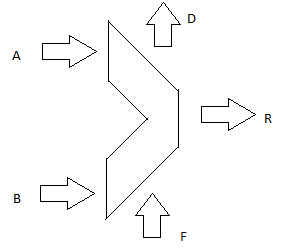
\includegraphics[]{images/ULA.png}
\caption{Desenho esquemático de uma ULA.}
\label{fig:ula}
\end{figure}

Nela, é possível ver que a ULA possui duas entradas e uma saída de dados,~\textit{A}, \textit{B} e~\textit{R} respectivamente, além de uma entrada e uma saída de sinais de controle,~\textit{F} e~\textit{D}.
As entradas \textit{A} e~\textit{B} são os valores que a ULA recebe para fazer os cálculos necessários.
Esses valores podem vir de registradores ou podem ser imediatos: números absolutos, como nas instruções a seguir:

\begin{lstlisting}
Addi R1,R2,10
Sub R3,R4,R5
\end{lstlisting}

A instrução 1 soma o valor imediato 10 ao valor armazenado no registrador \textit{R2} e armazena no registrador \textit{R1}.
No caso dessa instrução, a entrada~\textit{A} na Figura~\ref{fig:ula} recebe o valor do registrador~\textit{R2}, a entrada~\textit{B} o valor do imediato (10) e a saída~\textit{R} terá o valor da soma, sendo que este valor será armazenado no registrador~\textit{R1}.
Já a instrução 2 subtrai o valor armazenado no registrador~\textit{R5} do valor armazenado em~\textit{R4} e armazena em~\textit{R3}, fazendo a operação

\begin{equation}
\label{eq1:sub-ula}
R3=R4-R5
\end{equation}

A entrada de sinais~\textit{F} é a entrada de controles da ALU.
Dentre esses sinais de controle está o que sinaliza se o valor na entrada de dados~\textit{B} é o valor vindo de um registrador ou um imediato.
Esse sinal controla um multiplexador para seleciona qual entrada irá passar para a ALU, a entrada vinda do banco de registradores ou a entrada vinda direto da instrução no caso de um imediato.

Já a saída de sinais~\textit{D}, são os sinais que a ALU indica, sendo eles se o resultado é zero, negativo e se houve~\textit{overflow} na operação.

\section{Implementação}

Esta seção fala da implementação da ULA em \textit{Verilog}.
Nela, mostramos como cada parte da ULA foi implementada além de decisões de projeto tomadas.

O módulo desenvolvido possui 5 entradas e duas saídas: \textit{OpA}, \textit{OpB}, \textit{Op}, \textit{RST}, \textit{CLK}, \textit{Res} e \textit{FlagReg} respectivamente.
O Apêndice~\ref{app:ULA} mostra o código.

As entradas \textit{OpA} e \textit{OpB} representam as entradas \textit{A} e \textit{B} da Figura~\ref{fig:ula}.
A entrada \textit{Op} indica qual operação a ALU vai fazer (Add, Sub, etc.) e faz parte da entrada \textit{F} na Figura~\ref{fig:ula}.
As saídas \textit{Res} e \textit{FlagReg} indicam, respectivamente o resultado da operação e o sinal de saída da ALU, na Figura~\ref{fig:ula}, as saídas \textit{R} e \textit{D} respectivamente.

Na implementação, as entradas \textit{OpA} e \textit{OpB} são de \textit{16 bits}, que, de acordo com a especificação do trabalho, é o tamanho dos registradores.
Aqui, apenas o \textit{OpB} pode ser um imediato.
Neste caso, o imediato possui apenas \textit{4 bits}, sendo necessário estender mais \textit{12 bits}.
Mais a frente será mostrado como e onde essa operação é feita.
A entrada \textit{Op} indica a operação a ser realizada e possui \textit{4 bits}, ou seja, a ALU implementada possui um máximo de 16 operações diferentes.
Pela especificação, apenas 11 operações foram utilizadas como mostrado na Tabela~\ref{tab:ULA}.

\begin{table}[h]
\centering
\begin{tabular}{| c | c | c |}
\hline
Código & Operação & Descrição\\
\hline
0 & Add & Adição com registradores \\
\hline
1 & Sub & Subtração com registradores \\
\hline
2 & Slti & Salto condicional com imediato \\
\hline
3 & And & \textit{And} binário \\
\hline
4 & Or & \textit{Or} binário  \\
\hline
5 & Xor & \textit{Xor} binário  \\
\hline
6 & Andi & \textit{And} binário com imediato \\
\hline
7 & Ori & \textit{Or} binário com imediato \\
\hline
8 & Xori & \textit{Xor} binário com imediato  \\
\hline
9 & Addi & Adição com imediato \\
\hline
10 & Subi & Subtração com imediato \\
\hline
\end{tabular}
\caption{Descrição das operações implementadas.}
\label{tab:ULA}
\end{table}
\captionsetup{font={footnotesize,rm},justification=centering,labelsep=period}%

A saída \textit{Res} possui \textit{16 bits}, assim como as entradas \textit{OpA} e \textit{OpB} já que é o resultado da operação e a saída \textit{FlagReg} possui \textit{3 bits}, um para cada sinal de saída como mostra a Tabela~\ref{tab:flags}.

\begin{table}[h]
\centering
\begin{tabular}{| c | c |}
\hline
Índice & Sinal\\
\hline
0 & \textit{Carry/Overflow}\\
\hline
1 & Negativo \\
\hline
2 & Zero\\
\hline
\end{tabular}
\caption{Sinais de saída da ULA.}
\label{tab:flags}
\end{table}
\captionsetup{font={footnotesize,rm},justification=centering,labelsep=period}%

\begin{appendices}
	\chapter{Módulo ULA}
	\label{app:ULA}
	\begin{lstlisting}[style={verilog-style}]
module ULA (OpA, OpB, Res, Op, FlagReg, CLK, RST);

	input CLK, RST;
	input [3:0] Op;
	input [15:0] OpA, OpB;
	output reg [15:0] Res;
	output reg [2:0] FlagReg;		// [Z N C]: Z=Zero; N=Neg; C=Carry/Overflow
	
	wire [15:0] invOpB;
	assign invOpB = ~OpB + 16'd1;

	parameter InsADD = 4'b0000;	// ADD	Res = OpA + OpB
	parameter InsSUB = 4'b0001;	//	SUB	Res = OpA - OpB
	parameter InsSLT = 4'b0010;	//	SLTI	Res = (OpA > OpB) ? 1 : 0
	parameter InsAND = 4'b0011;	//	AND 	Res = OpA & OpB
	parameter InsOR =  4'b0100;	//	OR 	Res = OpA | OpB
	parameter InsXOR = 4'b0101;	//	XOR 	Res = OpA ^ OpB
	
	parameter OverflowFlag	= 0;
	parameter NegFlag 		= 1;
	parameter ZeroFlag		= 2;
	
	always @(posedge CLK) begin
	 if (RST) begin
	  FlagReg = 3'b000;
	 end
	 else begin
	  case (Op)
	   InsADD: begin			
	    Res = OpA + OpB;
					
	    /* Zero check */
	    if (Res == 0)
		 FlagReg[ZeroFlag] = 1'b1;
	    else
	     FlagReg[ZeroFlag] = 1'b0;
	    /* Overflow check */
	    FlagReg[OverflowFlag] = (OpA[15] & OpB[15] & ~Res[15]) | (~OpA[15] & ~OpB[15] & Res[15]);
	    /* Negative check */
	    FlagReg[NegFlag] = Res[15];
	   end
	   InsSUB: begin			
	    Res = OpA + invOpB;
	    /* Zero check */
	    if (Res == 0)
	     FlagReg[ZeroFlag] = 1'b1;
	    else
	     FlagReg[ZeroFlag] = 1'b0;
	    /* Overflow check */
	    FlagReg[OverflowFlag] = (OpA[15] & invOpB[15] & ~Res[15]) | (~OpA[15] & ~invOpB[15] & Res[15]);
	    /* Negative check */
	    FlagReg[NegFlag] = Res[15];
	   end
	   InsSLT: begin
	    if (OpA > OpB)
	     Res = 16'd1;
	    else
	     Res = 16'd0;
	    /* Zero check */
	    if (Res == 0)
	     FlagReg[ZeroFlag] = 1'b1;
	    else
	     FlagReg[ZeroFlag] = 1'b0;
	    /* Overflow check */
	    FlagReg[OverflowFlag] = (OpA[15] & OpB[15] & ~Res[15]) | (~OpA[15] & ~OpB[15] & Res[15]);
	    /* Negative check */
	    FlagReg[NegFlag] = Res[15];
	   end
	   InsAND: begin			
	    Res = OpA & OpB;
	    /* Zero check */
	    if (Res == 0)
	     FlagReg[ZeroFlag] = 1'b1;
	    else
	     FlagReg[ZeroFlag] = 1'b0;
	    /* Overflow check */
	    FlagReg[OverflowFlag] = (OpA[15] & OpB[15] & ~Res[15]) | (~OpA[15] & ~OpB[15] & Res[15]);
	    /* Negative check */
	    FlagReg[NegFlag] = Res[15];
	   end
	   InsOR: begin			
	    Res = OpA | OpB;
	    /* Zero check */
	    if (Res == 0)
	     FlagReg[ZeroFlag] = 1'b1;
	    else
	     FlagReg[ZeroFlag] = 1'b0;
	    /* Overflow check */
	    FlagReg[OverflowFlag] = (OpA[15] & OpB[15] & ~Res[15]) | (~OpA[15] & ~OpB[15] & Res[15]);
	    /* Negative check */
	    FlagReg[NegFlag] = Res[15];
	   end
	   InsXOR: begin			
	    Res = OpA ^ OpB;
	    /* Zero check */
	    if (Res == 0)
	     FlagReg[ZeroFlag] = 1'b1;
	    else
	     FlagReg[ZeroFlag] = 1'b0;
	    /* Overflow check */
	    FlagReg[OverflowFlag] = (OpA[15] & OpB[15] & ~Res[15]) | (~OpA[15] & ~OpB[15] & Res[15]);
	    /* Negative check */
	    FlagReg[NegFlag] = Res[15];
	   end
	  endcase
	 end
	end
endmodule
	\end{lstlisting}
\end{appendices}

%%%%%%%%%%%%%%%%%%%%%%%%%%%%%%%%%%%%%%%%%%%%%%%%%%%%%%%%%%%%%%%%%%%%%%%%%%%%%%%%%%%%%%%%%%%%%%%%%%%%%%%%%%%%%%%%%%%%%%%%%%%%%%%%%%%
% Para mudar o nome da seo de referncias
%\renewcommand{\bibname}{Referncias}
%\renewcommand{\refname}{Referncias}

\bibliographystyle{unsrt}
\addcontentsline{toc}{section}{Referências}
\bibliography{references}


%%%%%%%%%%%%%%%%%%%%%%%%%%%%%%%%%%%%%%%%%%%%%%%%%%%%%%%%%%%%%%%%%%%%%%%%%%%%%%%%%%%%%%%%%%%%%%%%%%%%%%%%%%%%%%%%%%%%%%%%%%%%%%%%%%
%\appendix
%
%\pagebreak
%\section{Artigo submetido ao \textit{ACM Transactions on Interactive Intelligent Systems (TiiS)}}
%\label{sec-submissaoTIIS}

%\includegraphics{Figuras/RecSys12}


%\pagebreak
%\section{Artigo submetido ao \textit{ACM Recommender Systems 2012}}
%\label{sec-submissaoRecSys}

%\includegraphics{Figuras/RecSys12}



\end{document}

